%!TEX root = ./sujet-projet.tex

\chapter{Architecture}

\section{Introduction}
	Dans ce chapitre, vous devez fournir une description générale de l'architecture de votre système et décrire comment vous répondez aux exigences non-fonctionnelles énoncés précédemment dans la Section~\ref{section:non-fonctionnelles}.


\section{Vue physique}

Utilisez un diagramme de déploiement UML pour décrire l'architecture physique de l'application: les nœuds logiques, les protocoles de communication, le déploiement des artefacts logiciels (bibliothèques, autres logiciels, etc.).
N'oubliez pas de décrire votre diagramme.

Si l'architecture physique répond à une ou des exigences logicielles, n'oubliez pas de le mentionner.

\begin{figure}[!htbp]
\begin{center}

\caption{Diagramme de déploiement du système ``\projet{}''}

\end{center}
\end{figure} 

Utilisez également le diagramme de déploiement, mais au niveau instance, pour fournir des exemples de déploiement du système.

\begin{figure}[!htbp]
\begin{center}

\caption{Diagramme d'instances modélisant un déploiement possible du système ``\projet{}''}
\end{center}
\end{figure} 


\section{Vue du développement}
Utilisez le diagramme de paquetages UML pour décrire l'organisation du code source de votre application.
N'oubliez pas de le commenter.

Si l'architecture logique répond à une ou des exigences logicielles, n'oubliez pas de le mentionner.

\section{Vue logique}

Présentez ici les composant principaux du système.

\begin{figure}[!htbp]
\begin{center}
\caption{Diagramme d'instances modélisant un déploiement possible du système ``\projet{}''}
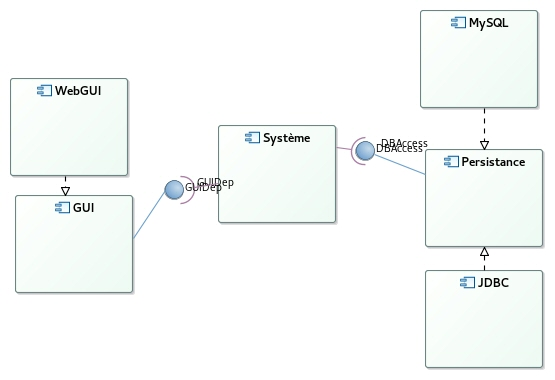
\includegraphics[scale=.7]{Vue_composants.jpg}
\end{center}
\end{figure} 

\section{Vue des processus}
Présentez ici les différents processus d'exécution dans votre système.

\section{Vue de la fiabilité}

Énumérez ici les choix architecturaux faits pour assurer la fiabilité du système.


\section{Réponses aux exigences non-fonctionnelles}
Expliquez, dans cette section, la réponse de votre solution aux exigences non-fonctionnelles. 
Les sous-sections présentées ici ne constituent pas une liste exhaustive. 

\subsection{Gestion de la concurrence}

\subsection{Gestion de la persistance}

\subsection{Gestion de la sécurité}


\section{Architecture technique : traduction de UML en code source}
Expliquez, dans cette partie, l'ensemble de règles que vous utiliserez par la suite pour traduire nos diagrammes \textsc{UML} (découlant de notre analyse et de notre conception) en code source (classes d'implémentation).\\ 

\subsection{Règles de traduction des types de base}

\subsection{Règles de traduction des classes}

\subsection{Règles de traduction des associations, agrégations composites et agrégations partagées}

\subsection{Règles de traduction des composants}

\subsection{Autres règles}



\section{Patrons architecturaux utilisés}

Fournissez, dans cette dernière partie, une liste exhaustive des patrons de conception que vous allez utiliser pour mettre en œuvre notre application. 
Pour chacun de ces patrons, donnez une courte description ainsi que les raisons pour lesquelles vous avez choisi de les mettre en \oe uvre.\\


\subsection{Patron A}

\subsection{Patron B}

\subsection{Patron C}

\subsection{Patron D}

\subsection{Patron D}

\subsection{Patron E}


\section{Choix techniques - Distribution des processus}

\indent Nous allons ici expliciter les différents choix techniques que nous avons choisit et les réponses technologiques aux différentes contraintes que notre système implique. Nous allons donc vous présenter l'environnement général de développement puis énoncer les 4 contraintes que nous avons déterminées de notre logiciel.

%
%  Choix de l'environnement  
%



\section{Conclusion}

